In the preceding lectures, we have discussed the task of classical message transmission over discrete memoryless quantum channels. We noticed, that 
we end up with a so-called multi-letter formula for the corresponding capacity which turns out as very unsatisfactory when it comes to calculating capacities. \newline
A very interesting scenario arises, if sender and receiver have access to shared entanglement in addition to the quantum channel. In case, 
that enough entanglement is present, the corresponding capacity turns out to be described by a single-letter formula, as we will see in this chapter. 
After all, the capacity formula we derive shows, that sometimes entanglement helps to achieve higher classical message transmission capacities for 
channel transmission. This may be regarded as somewhat surprising, since shared entanglement is not sufficient as resource for any nontrivial transmission
of classical messages. \newline 
Before we introduce precise definitions for the above mentioned coding scenario, we provide ourselves with a formalized evidence for the claim ``shared entanglement 
alone does not suffice for message transmission''. \newline 
Let $A$ denote the sending party, while $B$ is the receiver. Assume, the share a state $\rho \in \cS(\cK_A \otimes \cK_B)$. The most general way to set up a message 
transmission scheme for a number of $M$ messages is to assign a c.p.t.p. map 
$% \begin{align}
 \cE_m: \cL(\cK_A) \rightarrow \cL(\cH_A) \
$% \end{align} 
with any Hilbert space $\cH_{A'}$, and a matrix $D_m$, $0 \leq D_m \leq \bbmeins_{\cH_B}$ for each $m \in [M]$, such that $\sum_{m=1}^M D_m = \bbmeins_{\cH_B}$. Assume,
that 
\begin{align*}
 \cE_m(a) = \sum_{k=1}^K A_k a A_k^\ast &&(a \in \cL(\cK_A)) 
\end{align*}
is any Kraus decomposion for $\cE_m$. The probability, that $m'$ is received, while $m$ was sent, is given by 
\begin{align*}
 p(m'|m) \ 
 &  = \ \tr (\bbmeins_{\cH_A} \otimes D_{m'})(\cE_m \otimes \id_{\cH_B}(\rho)) \\
 &  = \ \sum_{k=1}^K \tr (\bbmeins_{\cH_A} \otimes D_{m'})(A_k \otimes \bbmeins_{\cH_B})(\rho)(A_k \otimes \bbmeins_{\cH_B})^\ast \\
 %&  = \ \sum_{k=1}^K \trA_k^\ast A_k \otimes D_{m'}\rho \\
 &  = \ \tr \left(\sum_{k=1}^K A_k^\ast A_k \right) \otimes D_{m'} \rho \\
 &  = \ \tr D_{m'}\rho_B. 
\end{align*}
Inspection of the above chain of equalities shows, that the probability to receive $m'$ is \emph{independent of the sent $m$}. In consequence, if $m_1, m_2 \in [M]$ are any two 
distinct messages, and $p(m_1|m_1) \geq 1 - \lambda$ for some $\lambda \in [0,1]$, then 
\begin{align*}
 p(m_2|m_2) \ = \ 1 - \sum_{m \neq m_2} p(m|m_2) \ \leq \ 1 - p(m_1|m_2) \ = \ 1 - p(m_1|m_1) \ <  \ \lambda.
\end{align*}
It is therefore not possible, to transmit one of two messages with an error less than $\frac{1}{2}$, which can be also achieved if the receiver randomly guesses the message. \\
Another "extreme" case arises from using the ideal quantum channel $\id_{\cH}$ together with a pure maximally entangled state on $\cH \otimes \cH$. In this case, using the so-called \emph{dense coding protocol}\index{dense coding}, $d^2$ messages can be transmitted with perfect reliability, i.e. the 
message transmission capacity without entanglement assistance is exceeded by a factor of $2$! 
\begin{theorem}[Dense coding]\label{thm:dense_coding} \index{dense coding}
Let $\cH_A = \cH_B = \cK_B = \bbmC^d$, $\id$ the ideal channel mapping $\cH_A$ to $\cH_B$. There exists a family
$\{\hat{\cE}_{m}\}_{m=1}^{d^2} \subset \cC(\cH_A,\cH_A)$, and a POVM $\{\hat{D}_m\}_{m=1}^{d^2}$ such that 
with $\phi := \sqrt{d}^{-1} \sum_{k=1}^{d} e_k \otimes e_k \in \cH_A \otimes \cK_B$ for each $m,m' \in [d^2]$ 
\begin{align*}
p(m'|m) \ := \ \tr \left(\id \circ\hat{\cE}_m \otimes \hat{D}_{m'}\ket{\phi}\bra{\phi}\right) \ = \ \delta_{mm'}.
\end{align*}
\end{theorem}
To prove the above assertion, we will use the following proposition 
%************************************************************************************************
%
% The following lemma is identical to lemma \ref{unitary_basis} in the teleportation chapter!
%
%************************************************************************************************
\begin{lemma}\label{lemma:unitary_basis_dense_coding} 
	Let $d \in \bbmN$. There exists a family $\{v_i\}_{i=1}^{d^2} \subset \cL(\bbmC^d)$ of unitary matrices, such that the following properties hold. 
	\begin{enumerate}
		\item $\tr v_i^\ast v_k \ = \ d \delta_{ij}$ for all $i,j \in [d^2]$
		\item With $\phi := \sqrt{d}^{-1} \sum_{k=1}^d e_k \otimes e_k$ and $\phi_i := (v_i\otimes \bbmeins)\phi$ for each $i \in [d]$, it holds  \label{lemma:unitary_basis_dense_coding_2}
		\begin{enumerate}
			\item[\ref{lemma:unitary_basis_dense_coding_2}a.] $\braket{\phi_i, \phi_j}  \ = \ \delta_{ij}$ for all $i,j \in [d]$
			\item[\ref{lemma:unitary_basis_dense_coding_2}b.] $\sum_{i=1}^{d^2} \ket{\phi_i}\bra{\phi_i} \ = \ \bbmeins \otimes \bbmeins$.
		\end{enumerate}
	\end{enumerate}
\end{lemma}
\begin{proof}
	Let $\gamma: \{0,d-1\} \times \{0,d-1\} \rightarrow [d^2]$ be any bijection. We will show, that the matrices
	\begin{align*}
	v_i := v_{\gamma(r,s)} := \sum_{l=0}^{d-1} e^{-i2\pi s l /d} \ket{e_{l \ominus r}}\bra{e_l} &&(i \in [d^2]) 
	\end{align*}
	suffice the properties claimed in the lemma ($\ominus$ denotes the modulo-$d$ substraction). Unitarity of $v_1,\dots, v_{d^2}$ follows by straightforward calculation. To show the first claim of the lemma, 
	let $(r,s) = \gamma{-1}(j)$, $(r',s') = \gamma^{-1}(k)$. It holds
	\begin{align*}
	\tr v_k^\ast v_j \ 
	= \ \sum_{l,l'=0}^{d-1} e^{i2\pi'(s'l' - sl)/d} \delta_{r'r}\cdot \delta_{l'l} \
	= \ \sum_{l=0}^{d-1} e^{i2\pi(s'-s)l/d}  \delta_{rr'} \label{lemma:unitary_basis_4}
	\end{align*}
	We assume $r = r'$ and evaluate the right hand side of (\ref{lemma:unitary_basis_4}). If $s=s'$, one can directly see, that $j=k$, and 
	\begin{align*}
	\tr_{v_k^\ast v_j} = d.
	\end{align*}
	When $s \neq s'$, then 
	\begin{align*}
	\sum_{l=0}^{d-1} e^{i2\pi(s'-s)l/d} \ = \ \sum_{l=0}^{d-1} (e^{i2\pi(s'-s)/d})^l = 0
	\end{align*}
	To verify the rightmost of the above inequalites, we notice, that evaluating the geometric sum $\sum_l=0^{d-1} q^l$ with $q = e^{i2\pi(s'-s)/d}$ leads us to 
	\begin{align*}
	\sum_{l=0}^{d-1} (e^{i2\pi(s'-s)/d})^l = \frac{1 - e^{i2\pi(s-s')}}{1- e^{(s-s')/d}} = 0.
	\end{align*}
	We summarize
	\begin{itemize}
		\item $k \neq j \ \Rightarrow \ r \neq r' \vee s \neq s' \ \Rightarrow \tr v_k^\ast v_j = 0$
		\item $k = j \ \Rightarrow \ r = r' \wedge s=s' \ \Rightarrow \tr v_k^\ast v_j = d$
	\end{itemize}
	which shows the first claim. The remaining statements are rather straightforward applications of the first statement and are left as exercises. 
\end{proof}
\begin{proof}[Proof of Theorem \ref{thm:dense_coding}]
Define, using the family $\{v_m\}_{m=1}^{d^2}$ of unitaries from the preceding lemma,
\begin{align*}
\hat{\cE}_m(a) \ := \ v_m^\ast a v_m \in \cC(\cH_A,\cH_A) &&(a \in \cL(\cH)),
\end{align*}
and
\begin{align*}
\hat{D}_m \ := \ (\bbmeins_{\cH_{B}} \otimes v_m)\ket{\phi}\bra{\phi}(\bbmeins_{\cH_{B}} \otimes v_m)^\ast = \ket{\phi_m}\bra{\phi_m}
	\end{align*}
where $\phi_m$ is the maximally entangled vector corresponding to $v_m$ in Lemma \ref{lemma:unitary_basis_dense_coding}.
Notice, that $\cE_m\otimes \id_{\cH_B}(\ket{\phi}\bra{\phi}) = \ket{\phi_m}\bra{\phi_m}$. It is easy to see, that $\{\hat{D}_m\}_{m=1}^{d^2}$ is indeed a POVM. Moreover, it holds
\begin{align*}
p(m'|m) \ 
&= \tr \left(\id \circ\hat{\cE}_m \otimes \hat{D}_{m'}\ket{\phi}\bra{\phi}\right) \\
&= \tr \hat{D}_{m'} \ket{\phi_m}\bra{\phi_m} \\
&= |\braket{\phi_m, \phi_{m'}}|^2\\
&= \delta_{mm'}
\end{align*}
which proves the claim.
\end{proof}
The main goal of this lecture is to give a characterization of the optimal asymptotical classical message transmission rates over a DMQ channel if sender and receiver can choose an arbitrary pure entangled state to assist coding.  \newline 
The general coding sheme for entanglement-assisted classical message transmission 
\index{classical message transmission!entanglement-assisted} over $n$ uses of a DMQC $\cN$ with assistance of a and a shared pure state $\Psi = \ket{\psi}\bra{\psi}$ is depicted below. 
\begin{center}
	\vspace{2ex}
	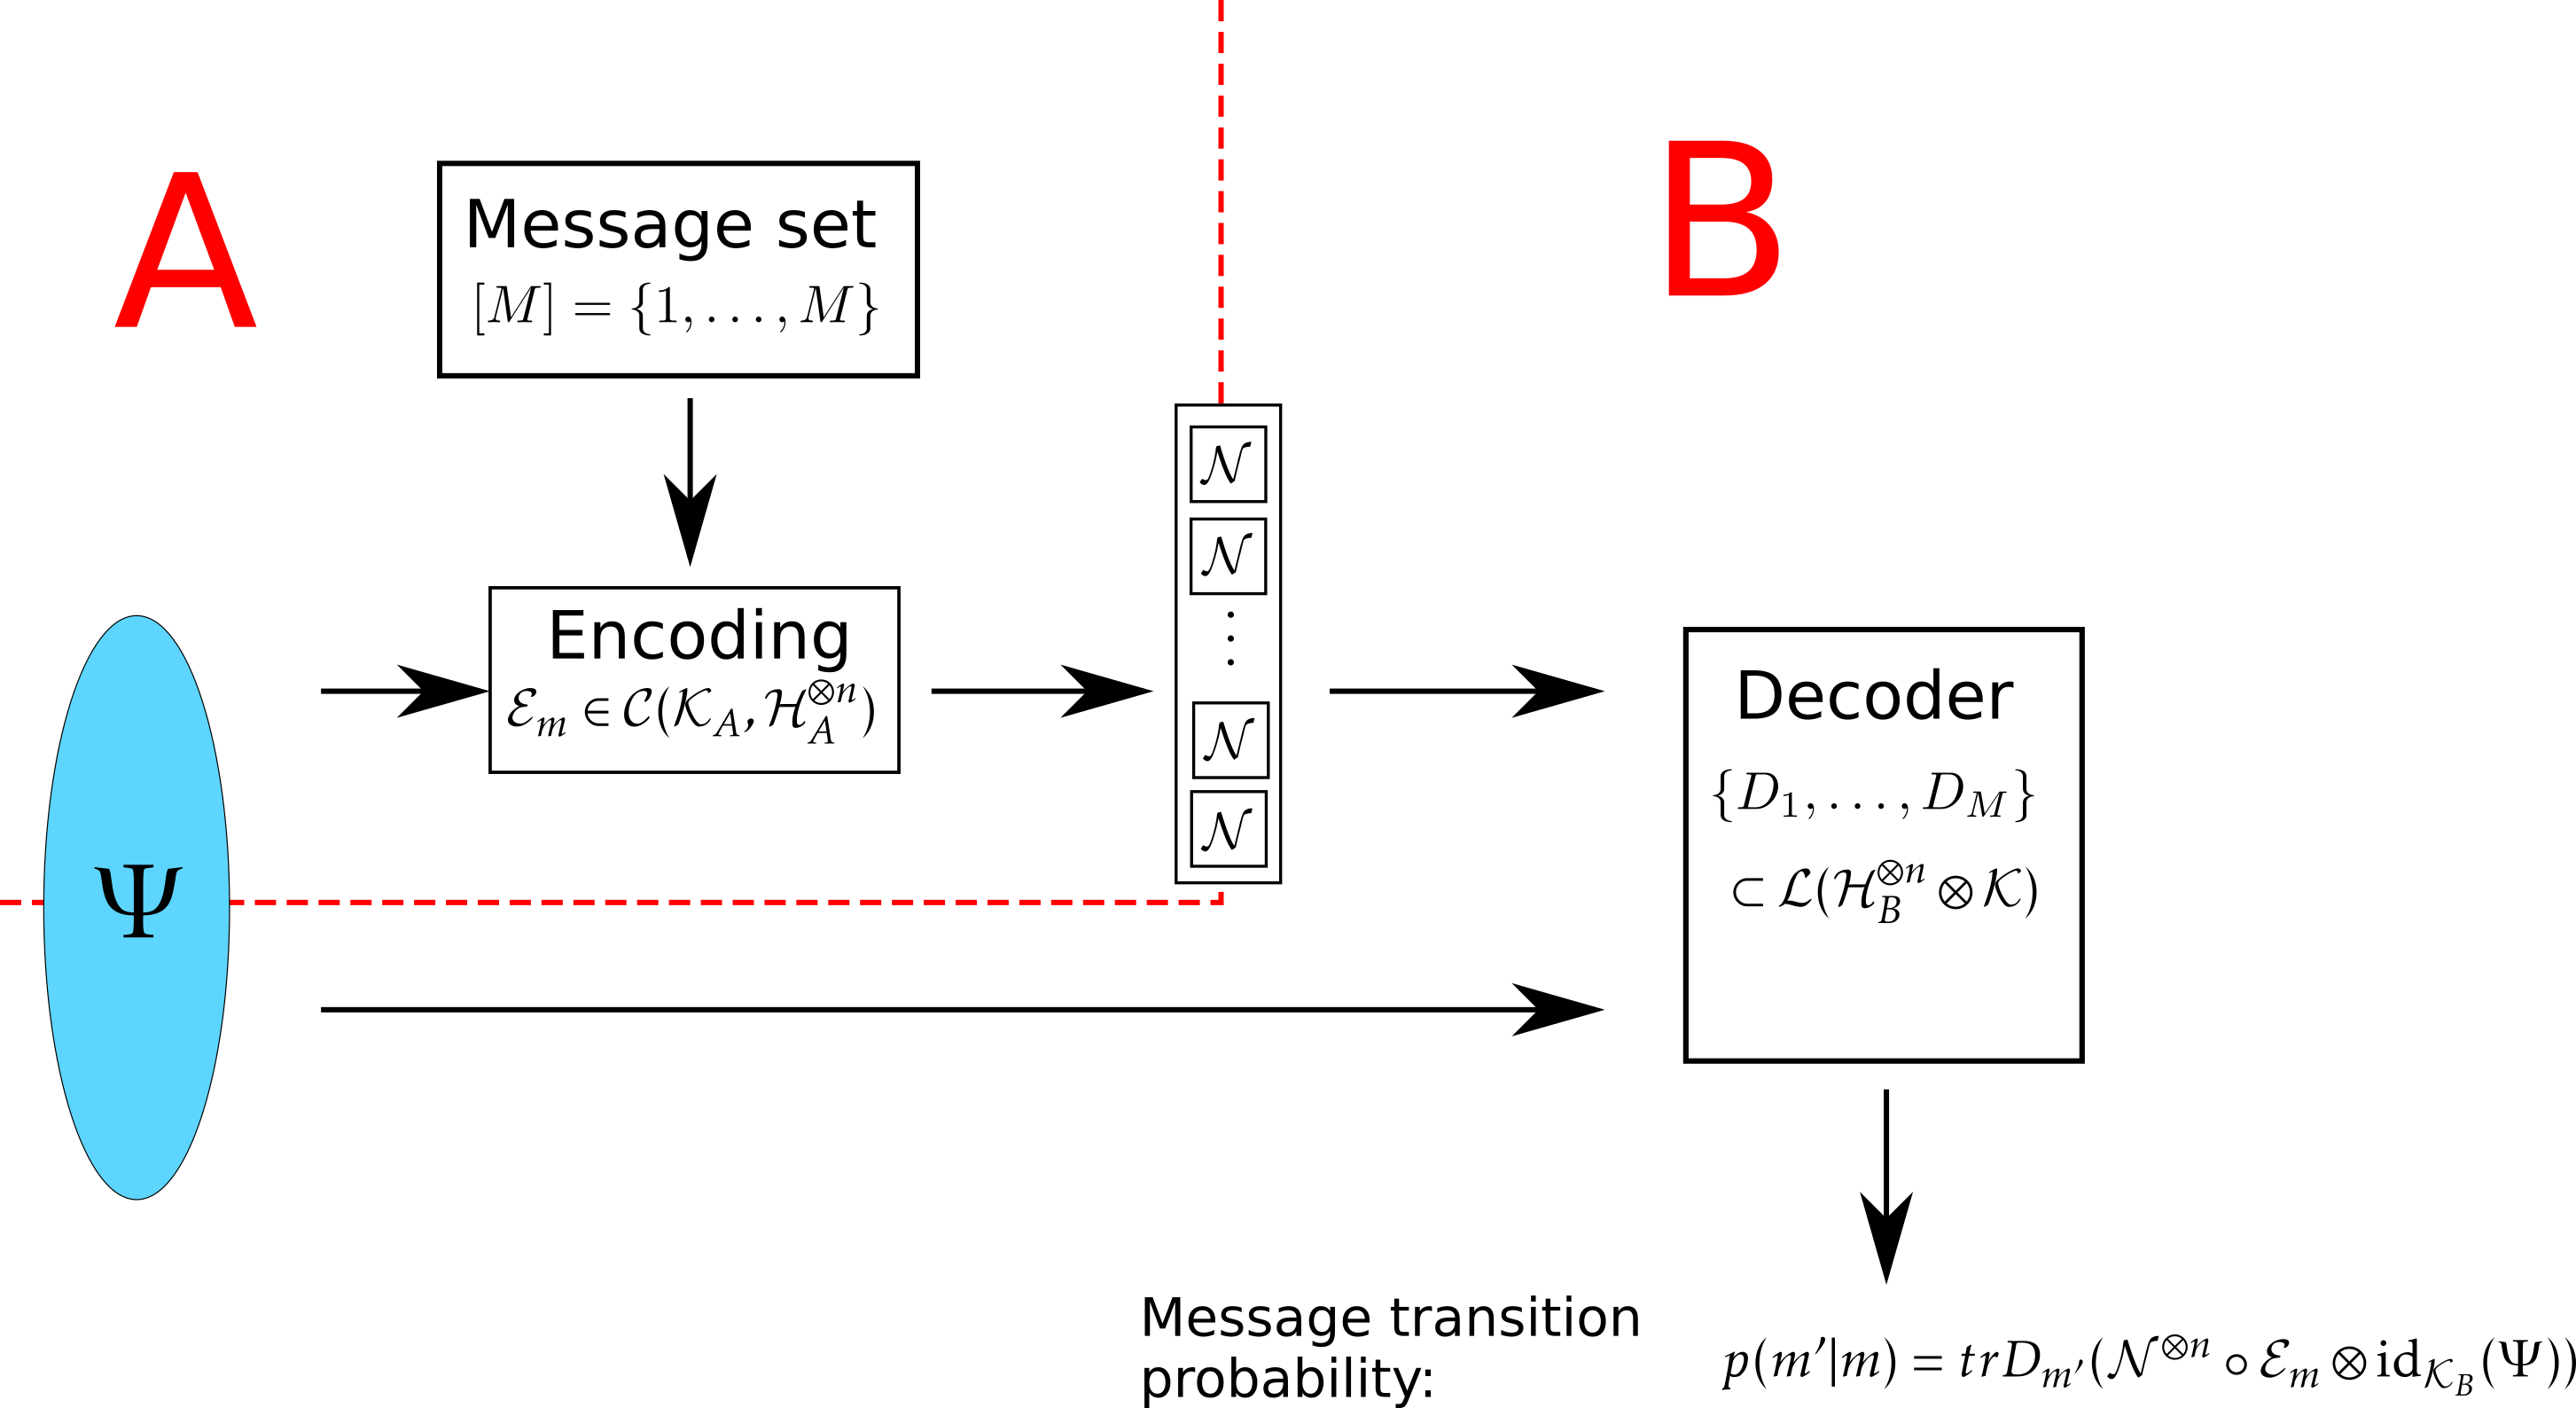
\includegraphics[scale=.8]{pics/entanglement_assisted_coding}
	\vspace{2ex}
\end{center}
We aim to determine the optimal asymptotically achievable message transmission rates in the above scenario. First we give the precise definitions. We fix the abbreviation ``EA'' for ``entanglement-assisted''.
\begin{definition}\label{def:ea_cl_mes_code}
Let $\cN \in \cC(\cH_A \otimes \cH_B)$ be a c.p.t.p. map. An \emph{$(n,M)$-EA message transmission code} for $\cN$ is a family $\cC := (\Psi, \cE_m, D_m)_{m=1}^M$ where
\begin{itemize}
 \item $\Psi := \ket{\psi}\bra{\psi} \in \cS(\cK_A \otimes \cK_B)$ is a pure state shared by sender and receiver. 
 \item $\cE_m \in \cC(\cK_A, \cH_A^{\otimes n})$ is a c.p.t.p. map for each $m \in [M]$, and
 \item $D_m \in \cL(\cH_B^{\otimes n}, \cK_B)$ is a matrix, such that $0 \leq D_m \leq \bbmeins_{\cH_B^{\otimes n} \otimes \cK_B}$, and $\sum_{m=1}^M D_m = \bbmeins_{\cH_B^{\otimes n} \otimes \cK_B}$.
\end{itemize}
\end{definition}
The \emph{average error} of the code $\cC$ is defined by 
\begin{align}
 \overline{e}_{EA}(\cC, \cN^{\otimes n}) \ := \ \frac{1}{M} \sum_{m=1}^M \ \tr D_m^c(\cN^{\otimes n} \circ \cE_m \otimes \id_{\cK_B}(\Psi)),
\end{align}
where we defined, with some abuse of notation $A^c := \bbmeins - A^c$ for each matrix $A$. As we did in case of classical message transmission without entanglement assistance, we define 
\begin{align*}
\overline{N}_{EA}(\cN, n , \epsilon) \ := \ \max\left\{M: \ \exists \ (n,M) \text{- EA message transm. code} \ \cC \ \text{s.t.} \ \overline{e}_{EA}(\cC, \cN^{\otimes n}) \leq \epsilon \right\} 
\end{align*}
for each $\epsilon \in [0,1]$ and $n \in \bbmN$. To state the corresponding capacity theorem, we introduce another quantum entropic quantity. 
\begin{definition}[Quantum mutual information] \index{quantum mutual information}
For a c.p.t.p. map $\cN \in \cC(\cH_A, \cH_B)$ and a state $\rho \in \cS(\cH_A)$, the \emph{quantum mutual information} \index{mutual information!quantum} is defined by
\begin{align}
 I(\rho,\cN) \:= S(\rho) + S(\cN(\rho)) - S(\cN \otimes \id_{\cK}(\ket{\psi}\bra{\psi})), \label{def:qmi_q}
\end{align}
where $\psi$ is the state vector of any purification of $\rho$. 
\end{definition}
\begin{remark}
Notice, that the term on the r.h.s. of Eq (\ref{def:qmi_q}) above is indeed independent of the choice of 
purification.
\end{remark}
\begin{theorem}[Entanglement-assisted capacity]\label{thm:ea_capacity}
Let $\cN \in \cC(\cH_A, \cH_B)$. It holds
\begin{enumerate}
 \item $\forall \epsilon > 0: \ \liminf_{n \rightarrow \infty} \frac{1}{n} \log \overline{N}_{EA}(\cN,n, \epsilon) \ \geq \sup_{\rho \in \cS(\cH_A)} I(\rho, \cN)$, and \label{thm:ea_capacity_1}
 \item $\inf_{\epsilon > 0}: \ \limsup_{n \rightarrow \infty} \frac{1}{n} \log \overline{N}_{EA}(\cN,n, \epsilon) \ \leq \sup_{\rho \in \cS(\cH_A)} I(\rho, \cN)$.  \label{thm:ea_capacity_2}
\end{enumerate}
\end{theorem}
\begin{exercise}
 Convince yourself, that the EA message transmission capacity is the same, when the maximal error criterion is taken into account instead of the average error. 
\end{exercise}
The claims of Theorem \ref{thm:ea_capacity} determine the input-state maximized quantum mutual information as the \emph{entanglement-assisted classical capacity} of the QDMC $\cN$.
Before we prove the claims of the above 
The following proposition states existence of codes sufficient for proving Theorem \ref{thm:ea_capacity}.\ref{thm:ea_capacity_1}. 
\begin{proposition}\label{prop:ea_achiev_codes}
 Let $\cN \in \cC(\cH_A, \cH_B)$ be a c.p.t.p. map, and $\sigma \in \cS(\cH_A)$. For each $\epsilon > 0, \delta > 0$ exists a number $n_0$ such that for each $n > n_0$
 \begin{align*}
  \overline{N}_{EA}(\cN, n ,\epsilon) \ \geq \ \exp\left(n(I(\sigma, \cN) - \delta) \right).
 \end{align*}
\end{proposition}
The strategy to prove the above claim will be, to combine a number of instances of the channel, a given pure bipartite state and certain encoding maps to form an ``effective'' classical-quantum channel. 
Afterwards, it will turn out, that classical message transmission codes for this cq channel can be reformulated to give EA message transmission codes for the original channel again. To support this strategy, we need the following lemma. 
\begin{lemma} \label{lemma:ea_mutual_holevo_approx}
 Let $\cH$ be a Hilbert space, $\dim \cH := d$, $\sigma \in \cS(\cH)$, and 
 \begin{align}
  \psi = \sum_{i=1}^d \sqrt{\alpha_i} v_i \otimes v_i
 \end{align}
 be a Schmidt decomposition of a purification $\psi$ of $\sigma$ ($\alpha_i = 0$ may occur for some $i$), and $k \in \bbmN$. There is a family 
 \begin{align}
  \{\tilde{\cE}_x\}_{x \in \cX} \subset \cC(\cH^{\otimes k}, \cH^{\otimes k}),
 \end{align}
 such that for each Hilbert space $\cK$, and each $\cN \in \cC(\cH, \cK)$ with the cq channel $V: \cX \rightarrow \cS(\cK^{\otimes n} \otimes \cK^{\otimes n})$,
 \begin{align}
  V(x) \ := \ \cN^{\otimes k} \circ \tilde{\cE}_x \otimes \id_{\cH}^{\otimes k}(\ket{\psi}\bra{\psi}^{\otimes k}) &&(x \in \cX)
 \end{align}
 The inequality 
 \begin{align}
  \left|k \cdot I(\rho,\cN) - \chi(q_\ast, V) \right| \ \leq \ 2 d \cdot \log(k+1) \label{lemma:ea_mutual_holevo_approx_1}
 \end{align}
 is fulfilled with $q_\ast$ being the equidistribution on $\cX$.
\end{lemma}
Before proving Lemma \ref{lemma:ea_mutual_holevo_approx}, we recall some properties of the typical sets. 
Let $\cX$ be an alphabet. For each $k \in \bbmN$, we define the set of \emph{$p$-typical words of lengths $k$} by 
\begin{align*}
T_p^k \ := \ \{x^k = (x_1,\dots,x_k): \forall a \in \cX: \frac{1}{k}N(a|x^k) = p(a)\},
\end{align*}
Where $N(a,x^k)$ is the number of occurencies of the letter $a$ in $x^k$. 
It is clear, that for some $p$, $k$, $T_p^k$ is empty. If $T_p^k$ is nonempty, we call 
$p$ a \emph{$k$-type}. We denote the set of all such $k$-types $\cT(\cX,k)$. By elementary counting arguments, it holds 
\begin{align}
|\cT(\cX,k)| \ \leq \ (k+1)^{|\cX|}, \label{type_counting}
\end{align}
i.e. the set of types on a given alphabet does at most increase polynomially with growing blocklengths.
Notice, that 
$
T_\lambda^k \cap T_\mu^k = \emptyset
$
for all $\lambda \neq \mu \in \cT(l,\cX)$. Moreover, 
\begin{align}
\bigcup_{\lambda \in \cT(\cX,k)} T_\lambda^k \ = \ \cX^k. \label{type_collection}
\end{align} 
Summarizing the above relations, we notice that \emph{the collection of sets of typical $k$-words form a disjoint decomposition of} $\cX^k$
The concept of types can be adopted to the quantum setting as follows. Let $\sigma \in \cS(\cH)$ be a given quantum state, and 
\begin{align*}
 \sigma \ = \ \sum_{x \in \cX} \alpha_x \ket{\tau_x}\bra{\tau_x} 
\end{align*} 
be a spectral decomposition of $\sigma$ with an orthonormal basis $\{\tau_x\}_{x \in \cX}$ in $\cH$, $|\cX| = \dim \cH$.
We regard $\alpha$ as a probability distribution on $\cX$ with $\alpha(x) = \alpha_x$. By the properties 
of types and sets of typical words, the collection $\{\cH_\lambda: \lambda \in \cT(\cX,k)\}$ with
\begin{align*}
\cH_\lambda \ := span \{\tau_{x^k} := \tau_{x_1}\otimes \cdots \otimes \tau_{x_k}: \ x^k \in T_\lambda^k\}
\end{align*}
is a collection of mutually orthogonal subspaces of $\cH$ such that $\cH^{\otimes k}$ can be written as a direct sum
of these spaces, i.e. 
\begin{align*}
\cH^{\otimes k} \ = \ \bigoplus_{\lambda \in \cT(\cX, k)} \cH_\lambda.
\end{align*}
Note, that by construction $\dim \cH_\lambda = |T_\lambda^k|$ for each $k$-type $\lambda$. \\
We are now ready for the proof of Lemma \ref{lemma:ea_mutual_holevo_approx}. 
\begin{proof}[Proof of Lemma \ref{lemma:ea_mutual_holevo_approx}]
We fix a blocklength $k$ and abbreviate $\cT_k := \cT(\cX,k)$. Using the Schmidt decomposition of $\psi$
from the hypotheses of the lemma, we write 
\begin{align*}
\psi^{\otimes n} \ 
&= \ \sum_{x^k \in \cX^k} \sqrt{\alpha^k(x^k)} \ \tau_{x^k} \otimes \tau_{x^k} \\
&= \sum_{\lambda \in \cT} \sum_{x^k \in T_\lambda^k} \sqrt{\alpha^k(x^k)} \ \tau_{x^k} \otimes \tau_{x^k}.
\end{align*}
For fixed $k$-type $\lambda$, the $\alpha^k$-probability is constant over the words in $T_\lambda^k$. It 
holds for each $x^k \in T_\lambda^k$
\begin{align*}
\alpha^k(x^k) = \frac{\alpha^k(T_\lambda^k)}{|T_\lambda^k|} =: \frac{\mu_{\lambda}}{|T_\lambda^k|}.
\end{align*}
Therefore, we have with the definition 
\begin{align*}
\phi_\lambda := \frac{1}{\sqrt{|T_\lambda^k|}} \sum_{x^k \in T_\lambda^k} \tau_{x^k} \otimes \tau_{x^k}
\end{align*}
the relations
\begin{align}
\psi^{\otimes k} \
&= \ \sum_{\lambda \in \cT_k} \sum_{x^k \in T_\lambda^k} \sqrt{\alpha^k(x^k)} \ \tau_{x^k} \otimes \tau_{x^k} \nonumber \\
&= \ \sum_{\lambda \in \cT_k} \sqrt{\mu_\lambda}\cdot \frac{1}{\sqrt{|T_\lambda^k|}} \sum_{x^k \in T_\lambda^k} \tau_{x^k} \otimes \tau_{x^k} \nonumber \\
&= \ \sum_{\lambda \in \cT_k} \sqrt{\mu_\lambda}\cdot \phi_\lambda. \label{lemma:ea_mutual_holevo_approx_2}
\end{align}
It is critical to notice here, that for each $k$-type $\lambda$, $\phi_\lambda$ is a maximally entangled state vector on $\cH_\lambda \otimes \cH_\lambda$. For the calculations that follow, we define the shortcuts $d_\lambda := \dim \cH_\lambda$ and $\cY_\lambda := [d_\lambda^2] \times \{0,1\}$ for each $\lambda \in \cT_k$. \newline
Let for each type $\lambda$
\begin{align*}
\{v_{j_\lambda}^{\lambda} \}_{j_\lambda = 1}^{d_\lambda^2} \subset \cL(\cH_\lambda)
\end{align*}
be a family of unitaries as stated in Lemma \ref{lemma:unitary_basis_dense_coding}. We extend each of these to maps on $\cL(\cH^{\otimes n})$ via zero-padding, i.e. 
We define the action of $v_{j_\lambda}^{d_\lambda^2}$ on the orthocomplement of $\cH_\lambda$ by
\begin{align} 
v_{j_\lambda}^{\lambda} x  \ := \ 0 && (x \in \cH_\lambda^\perp)
\end{align}
Define $\cY \ = \ \prod_{\lambda \in \cT} \ \cY_\lambda$ (this is the cartesian product!), 
and for each $\lambda \in \cT_k$, $y_\lambda := (j_\lambda,r_\lambda) \in \cY_\lambda$
\begin{align*}
u_{y_\lambda}^\lambda \:=\ v_{j_\lambda}^\lambda \cdot (-1)^{r_\lambda}.
\end{align*}
We have, using the representation of $\psi^{\otimes k}$ from Eq. (\ref{lemma:ea_mutual_holevo_approx_2}) 
\begin{align}
(u_{y_\lambda}^{\lambda} \otimes \bbmeins^{\otimes k}) \psi^{\otimes k} \ 
= \ \sum_{\gamma \in \cT} \sqrt{\mu_\gamma} (u_{y_\lambda}^{\lambda} \otimes \bbmeins^{\otimes k}) \phi_\gamma  
\ = \ \sqrt{\mu_\lambda}(u_{y_\lambda}^{\lambda} \otimes \bbmeins^{\otimes k}) \phi_\lambda.
\end{align}
The rightmost of the above equalities is by the fact, that $(u_{y_{\lambda}}^\lambda \otimes \bbmeins^{\otimes k})\phi_{\gamma} = \delta_{\gamma \lambda} \phi_\gamma$. We define for each $y = (y_\lambda)_{\lambda \in \cT_k} \in \cY$
\begin{align*}
u_y \ := \ \sum_{\lambda \in \cT_k} u_{y_\lambda}^\lambda, 
\end{align*}
and $\tilde{\cE}_y(a) \ := \ u_y(a)u_y^\ast$ for each $y \in \cY$. Therefore, we have for all $y = (y_\lambda)_{\lambda \in \cT_k}$ 
\begin{align*}
\tilde{\cE_y} \otimes \id_{\cH}^{\otimes k}(\ket{\psi}\bra{\psi}^{\otimes k}) \ 
&= \ \sum_{\lambda, \gamma \in \cT_k} (u_{y_\lambda}^\lambda \otimes \bbmeins^{\otimes k}) \ket{\psi}\bra{\psi}^{\otimes k}(u_{y_\gamma}^\gamma \otimes \bbmeins^{\otimes k})^\ast \\ 
&= \ \sum_{\lambda, \gamma \in \cT_k} (u_{y_\lambda}^\lambda \otimes \bbmeins^{\otimes k}) \ket{\phi_\lambda}\bra{\phi_\gamma}(u_{y_\gamma}^\gamma \otimes \bbmeins^{\otimes k})^\ast. 
\end{align*}
To proceed with the proof we need to show two identities. \\
\begin{align*}
  \text{Identity 1:} \hspace{2cm} \frac{1}{|\cY|} \sum_{y \in \cY} \tilde{\cE}_y \otimes \id_{\cH}^{\otimes k}(\ket{\psi}\bra{\psi}^{\otimes k}) \ = \ \sum_{\lambda \in \cT} \ \mu_\lambda \pi_\lambda \otimes \pi_\lambda,
\end{align*}
where $\pi_\lambda = \frac{\bbmeins_{\cH_\lambda}}{d_\lambda}$ is the maximally mixed state on $\cH_\lambda$ for each type $\lambda$. To prove the above equation, we consider the sum
\begin{align*}
 \frac{1}{|\cY|}\sum_{y \in \cY} (\tilde{\cE}_y \otimes \id_{\cH}^{\otimes k})(\ket{\psi}\bra{\psi}^{\otimes k}) \
 & = \frac{1}{|\cY|}\sum_{y \in \cY}\sum_{\lambda, \gamma \in \cT_k} 
	   \sqrt{\mu_\lambda\cdot \mu_\gamma} (u_{y_\lambda}^\lambda \otimes \bbmeins_{\cH}^{\otimes k})\ket{\psi}\bra{\psi}^{\otimes k}(u_{y_\gamma}^\gamma \otimes \bbmeins_{\cH}^{\otimes k})^\ast \\
 & = \frac{1}{|\cY|}\sum_{y \in \cY}\sum_{\lambda, \gamma \in \cT_k} 
 \sqrt{\mu_\lambda\cdot \mu_\gamma} (u_{y_\lambda}^\lambda \otimes \bbmeins_{\cH}^{\otimes k})\ket{\phi_\lambda}\bra{\phi_\gamma}(u_{y_\gamma}^\gamma \otimes \bbmeins_{\cH}^{\otimes k})^\ast 
 \end{align*}
  We evaluate the inner sums in the last line above for two cases. 
  \begin{itemize}
  	\item $\lambda \neq \gamma$: We have
  	\begin{align*}
     & \sum_{y \in \cY} 
     \sqrt{\mu_\lambda\cdot \mu_\gamma} (u_{y_\lambda}^\lambda \otimes \bbmeins_{\cH}^{\otimes k})\ket{\phi_\lambda}\bra{\phi_\gamma}(u_{y_\gamma}^\gamma \otimes \bbmeins_{\cH}^{\otimes k})^\ast \\
     &= \left(\frac{|\cY|}{|\cY_\lambda|}\right)^2\sum_{y_\lambda \in \cY_\lambda}\sum_{y_\gamma \in \cY_\gamma}
     \sqrt{\mu_\lambda\cdot \mu_\gamma} (u_{y_\lambda}^\lambda \otimes \bbmeins_{\cH}^{\otimes k})\ket{\phi_\lambda}\bra{\phi_\gamma}(u_{y_\gamma}^\gamma \otimes \bbmeins_{\cH}^{\otimes k})^\ast \\
     &= \ \left(\frac{|\cY|}{|\cY_\lambda|}\right)^2 \sum_{r_\lambda, r_\gamma \in \{0,1\}} (-1)^{r_\lambda + r_\gamma} \sum_{j_\lambda \in [d_\lambda^2]} \sum_{j_\gamma \in [d_\gamma^2]}
     \sqrt{\mu_\lambda\cdot \mu_\gamma} (v_{j_\lambda}^\lambda \otimes \bbmeins_{\cH}^{\otimes k})\ket{\phi_\lambda}\bra{\phi_\gamma}(v_{j_\gamma}^\gamma \otimes \bbmeins_{\cH}^{\otimes k})^\ast \\
  	& = \ 0
  	\end{align*} 
  	The last inequality above is by the fact, that $\sum_{r_\lambda, r_\gamma \in \{0,1\}} (-1)^{r_\lambda + r_\gamma}$ vanishes.
    \item $\lambda = \gamma$. In this case, The inner sum reads
    \begin{align*} 
     & \sum_{y \in \cY}
     \mu_\lambda (u_{y_\lambda}^\lambda \otimes \bbmeins_{\cH}^{\otimes k})\ket{\phi_\lambda}\bra{\phi_\lambda}(u_{y_\lambda}^\lambda \otimes \bbmeins_{\cH}^{\otimes k})^\ast  \\
     &= \frac{|\cY|}{|\cY_\lambda|}\sum_{y_\lambda \in \cY_\lambda}
     \mu_\lambda (u_{y_\lambda}^\lambda \otimes \bbmeins_{\cH}^{\otimes k})\ket{\phi_\lambda}\bra{\phi_\lambda}(u_{y_\lambda}^\lambda \otimes \bbmeins_{\cH}^{\otimes k})^\ast  \\
     & = \frac{|\cY|}{|\cY_\lambda|}  \ \sum_{r_\lambda} (-1)^{2 \cdot r_\lambda} \sum_{j_\lambda \in [d_\lambda^2]} 
     \mu_\lambda (v_{j_\lambda}^\lambda \otimes \bbmeins_{\cH}^{\otimes k})\ket{\phi_\lambda}\bra{\phi_\lambda}(v_{j_\lambda}^\lambda \otimes \bbmeins_{\cH}^{\otimes k})^\ast \\
     & = \frac{|\cY|}{|\cY_\lambda|}2 \mu_\lambda \cdot \bbmeins_{\cH}^{\otimes k} \otimes \bbmeins_{\cH}^{\otimes k} \\
     & = \frac{|\cY|}{|\cY_\lambda|}2 d_\lambda^2 \mu_\lambda \pi_\lambda \otimes \pi_\lambda \\
     & = |\cY| \mu_\lambda \pi_\lambda \otimes \pi_\lambda.
    \end{align*} 
  \end{itemize} 
The second identity is
\begin{align*}
    \text{Identity 2:} \hspace{1cm} (\cN \circ \tilde{\cE}_y \otimes \id_{\cH}^{\otimes k})(\ket{\psi}\bra{\psi}^{\otimes k})  \ 
  = \ (\bbmeins^{\otimes k} \otimes u_y^T)\cN \otimes \id_{\cH}^{\otimes k}(\ket{\psi}\bra{\psi}^{\otimes k})(\bbmeins^{\otimes k} \otimes u_y^T)^\ast
\end{align*}
holding for any given c.p.t.p. map $\cN \in \cC(\cH^{\otimes k}, \cK)$ with a Hilbert space $\cK$. To prove Identity 2, we remember the claim of Lemma \ref{lemma:entanglement_trick} from Chapter \ref{chap:source_comp}. If $\phi$ is the state vector of a maximally entangled pure state on $\cF \otimes \cF$, and $A$ a matrix on $\cF$, then
\begin{align*}
(\bbmeins_{\cF} \otimes A)\phi \ = \ (A^T \otimes \bbmeins_{\cF})\phi.
\end{align*}
This fact applied on each $\lambda \in \cT_k$ together with the representation in (\ref{lemma:ea_mutual_holevo_approx_2}) proves the claim. \newline 
From Identity 2 and unitary invariance of the von Neumann entropy, we directly obtain 
\begin{align}
S(\cN \circ \tilde{\cE}_y \otimes \id_{\cH}^{\otimes k}(\ket{\psi}\bra{\psi}^{\otimes k})) \
= \ S(\cN \otimes \id_{\cH}^{\otimes k}(\ket{\psi}\bra{\psi}^{\otimes k}))
\end{align}
Having these equalities, we can calculate
\begin{align*}
S\left(\frac{1}{|\cY|} \sum_{y \in \cY} \cN^{\otimes k} \circ \tilde{\cE}_y \otimes \id_{\cH}^{\otimes k} (\ket{\psi}\bra{\psi}^{\otimes k})\right) \ 
& = \ S\left(\cN^{\otimes k} \otimes \id_{\cH}^{\otimes k}\left(\sum_{\lambda \in \cT} \mu_\lambda \pi_\lambda \otimes \pi_\lambda\right)\right) \\
& \geq  \sum_{\lambda \in \cT_k} \mu_\lambda S(\cN^{\otimes k} \otimes \id_{\cH}^{\otimes k}(\pi_\lambda \otimes \pi_\lambda)) \\
& = \sum_{\lambda \in \cT_\lambda} \mu_\lambda \left( S(\cN^{\otimes k}(\pi_k)) + S(\pi_\lambda)\right)\\
& \geq S\left(\cN^{\otimes k}\left(\sum_{\lambda \in \cT_k} \mu _\lambda \pi_\lambda\right)\right) 
 \ + \ S\left(\sum_{\lambda \in \cT_k} \mu _\lambda \pi_\lambda\right)  
 - 2\ H(\mu) \\ 
& \geq S(\cN(\sigma)^{\otimes k}) \ + \ S(\sigma^{\otimes k}) - d \cdot \log(k+1)
\end{align*}
The first inequality above is by concavity, the second by almost-convexity of the von Neumann entropy (Lemma \ref{lemma:s_almost_convexity}). The last inequality is by our initial representation of $\sigma^{\otimes k}$ in terms of mutually orthogonal projections onto typical subspaces together with the bound $H(\mu) \leq \log |\cT_k| \leq d \cdot \log(k+1)$. \newline 
Choosing $q_\ast$ and $V$ as in the hypotheses of the proposition, we have
\begin{align*}
  \chi(q_\ast, V) \ 
  & = \ S\left(\frac{1}{|\cY|} \sum_{y \in \cY} \cN{\otimes k} \circ \tilde{\cE}_y \otimes \id_{\cH}^{\otimes k} (\ket{\psi}\bra{\psi}^{\otimes k})\right) 
  \ - \ \frac{1}{|\cY|} \sum_{y \in \cY} \ S(\cN^{\otimes k} \circ \tilde{\cE}_y \otimes \id_{\cH}^{\otimes k}(\ket{\psi}\bra{\psi}^{\otimes k})) \\
  & \geq \ S(\cN(\sigma)^{\otimes k}) \ + \ S(\sigma^{\otimes k}) - d \cdot \log(k+1)
    - S(\cN^{\otimes k} \otimes \id_{\cH}^{\otimes k}(\ket{\psi}\bra{\psi}^{\otimes k})) \\
  & = \ k \cdot I(\sigma, \cN) \ - \ d \cdot \log(k+1)
\end{align*}
The reversed inequality can be proven in a similar way.
\end{proof}
Now we are ready to prove Proposition \ref{prop:ea_achiev_codes}. 
\begin{proof}[Proof of Proposition \ref{prop:ea_achiev_codes}]
Set $d_A := \dim \cH_A$, $d_B := \dim \cH_B$, and fix a state $\sigma \in \cS(\cH_A)$. Let
\begin{align*}
\sigma \ = \ \sum_{i=1}^{d_A} \alpha_i \tau_i
\end{align*}
be a spectral decomposition of $\sigma$. Define a pure state $\Psi := \ket{\psi}\bra{\psi} 
\in \cS(\cH_A \otimes \cH_A)$ via
\begin{align*}
\psi := \sum_{i=1}^{d_A} \sqrt{\alpha_i} \tau_i \otimes \tau_i.
\end{align*}
Let $\{\tilde{\cE}\}_{x \in \cX}$ be a family of channels as in Lemma \ref{lemma:ea_mutual_holevo_approx}. Define the cq channel $V: \cX \rightarrow \cS(\cH_B^{\otimes k}\otimes \cH_B^{\otimes k})$ by
\begin{align*}
V(x) \ := \ \cN^{\otimes k} \circ \tilde{\cE}_x \otimes \id_{\cH_B}^{\otimes k}(\Psi^{\otimes k})&& (x \in \cX).
\end{align*}
With Lemma \ref{lemma:ea_mutual_holevo_approx}, we know, that 
\begin{align*}
\chi(q_\ast,V) \ \geq \ k I(\sigma,\cN) - d_A \log(k+1)
\end{align*}
holds. \newline 
Fix $\epsilon, \delta > 0$, and an arbitrary blocklength $n \in \bbmN$. Write $n = a\cdot k + b$ with $a, b \in \bbmN$, $0 \leq b < k$. If $a$ is large enough (which happens for large enough $n$), we have
\begin{align*}
 N(a, V, \epsilon) \ \geq \exp(a (\chi(q_\ast, V)- \frac{\delta}{2})).
\end{align*}
This follows from the achievability statement in Holevo's Theorem. Consequently, there is an $(a,M)$ code $\tilde{\cC} = (u_m, \tilde{D}_m)_{m=1}^M$ for classical message transmission over the DMCQ channel $V$ with 
\begin{align*}
 M \ \geq \ \exp\left(a(\chi(q_\ast, V) -\frac{\delta}{2})\right)
\end{align*}
and average transmission error
$
\overline{e}(\tilde{\cC}, V^{\otimes a}) \ \leq \ \epsilon.
$
We will now use $\tilde{\cC}$ to construct an $(n,M)$ code for entanglement-assisted message transmission over $\cN$. \newline 
Define, for each $m \in [M]$, and each codeword  $u_m = (u_{m,1},\dots, u_{m,a})$ from $\tilde{\cC}$ a c.p.t.p. map $\cE_m \in \cC(\cH_A^{\otimes n} \otimes \cH_A^{\otimes n})$ by
\begin{align*}
\cE_m(\cdot) \ := \ \tilde{\cE}_{u_{m,1}} \otimes \cdots \otimes \cE_{u_{m,a}} \otimes \id_{\cH}^{\otimes b}(\cdot),
\end{align*}
and a POVM $\{D_m\}_{m =1}^M$ on $(\cH_B \otimes \cH_B)^{\otimes n}$ by 
\begin{align*}
D_m \ := \ \tilde{D}_m \otimes \bbmeins_{\cH_B \otimes \cH_B}^{\otimes b}.
\end{align*}
With the preceding definitions, and the pure maximally entangled state $\Psi := \ket{\psi}\bra{\psi}$, $\cC := (\Psi,\cE_m,D_m)_{m=1}^M$ is an $(n,M)$-EA message transmission code for $\cN$. Moreover, it holds for each $m \in [M]$
\begin{align*}
 \tr D_m\left(\cN^{\otimes n} \circ \cE_m(\Psi^{\otimes n})\right) \ 
 & =\ \tr\tilde{D}_m(\bigotimes_{i=1}^a \cN^{\otimes k} \circ \tilde{\cE}_{u_{m,i}} \otimes \id_{\cH_B}^{\otimes k}(\Psi^{\otimes k})) \ \cdot \ \tr(\cN^{\otimes b}\otimes \id_{\cH_B}^{\otimes b}(\Psi^{\otimes b}))\\ 
 & = \tr \tilde{D}_m V^{\otimes a}(u_m).
 \end{align*}
 Arithmetic averaging of the above equality over all messages leads us to
 \begin{align*}
 \overline{e}_{EA}(\cC, \cN^{\otimes n}) \ = \ 1 - \frac{1}{M} \sum_{m=1}^M \tr \tilde{D}_m V^{\otimes a}(u_m) \ \leq \epsilon
 \end{align*}
 Therefore, 
 \begin{align}
 N(n, \cN, \epsilon) \ 
 & \geq \ M \nonumber \\
 &\geq \exp\left(a (\chi(q_\ast,V)-\frac{\delta}{2})\right) \nonumber \\
 &> \exp\left(n \left(\frac{1}{k} \chi(q_\ast,V) - \frac{\delta}{2k} - \frac{1}{kn}(\chi(q_\ast,V)\cdot \frac{\delta}{2k})\right) \right)  \label{fastende}
\end{align}
where the last inequality stems from 
\begin{align*}
a = \frac{n-b}{k} > \frac{n-k}{k} = \frac{n}{k(1 - \frac{1}{n})}.
\end{align*}
Evaluating the exponent on the right hand side of the inequality in (\ref{fastende}), we obtain using Lemma \ref{lemma:ea_mutual_holevo_approx}
\begin{align}
\frac{1}{k} \chi(q_\ast,V) - \frac{\delta}{2k} - \frac{1}{kn}(\chi(q_\ast,V)\cdot \frac{\delta}{2k}) \ 
 & \geq I(\sigma, \cN) - \frac{1}{k}(d_A \log(k+1)) - \frac{\delta}{2} - \frac{1}{n} \chi(q_\ast,V) - \frac{\delta}{2n}. \label{fastfastende}
\end{align}
If $n$ is large enough, we can infer from (\ref{fastende}) and (\ref{fastfastende}), that the claimed 
inequality 
\begin{align*}
\overline{N}_{EA}(n,\cN, \epsilon) \ \geq \ \exp(n(I(\sigma,\cN)- \delta))
\end{align*}
is fulfilled.
\end{proof}

\begin{lemma} \label{lemma:ent_ass_conv_pre}
	Let $\cN \in \cC(\cH_A, \cH_B)$, $\Psi \in \cS(\cH_A \otimes \cK_B)$ be a pure state, $\{\cE_m\}_{m=1}^{M} \subset \cC(\cH_A, \cH_A)$, and $q \in \cP([M])$. Define the c.p.t.p. map $\cE(\cdot) := \sum_{m\in [M]} q(m) \cE_m(\cdot)$, and $\rho_A \:= \ \tr_{\cK_B}\Psi$. With the cq channel $V:\ [M] \rightarrow \cS(\cH_B \otimes \cK_B)$,
	\begin{align*}
	 m \ \mapsto \ V(m) \ := \ \cN\circ \cE_m \otimes \id_{\cK_B}(\Psi),
	\end{align*}
	it holds 
	\begin{align}
	\chi(q,V) \ \leq \ I(\cE(\rho_A), \cN).  
	\end{align}
\end{lemma}
\begin{proof}
We introduce the shortcuts 
\begin{align*}
\tilde{\rho}_m \ := \ \cE_m \otimes \id_{\cK_B}(\Psi), \hspace{.5cm} \text{and} \hspace{.5cm} \rho_{B} \ := \ \tr_{\cK_A \Psi}
\end{align*}
for each $m \in [M]$. By subadditivity of the von Neumann entropy, we have 
\begin{align*}
\chi(q,V) \
&= \ S\left(\cN\circ \cE \otimes \id_{\cK_B}(\Psi)\right) 
 - \sum_{m=1}^M q(m) \ S(\cN \otimes \id_{\cK_B}(\tilde{\rho}_m)) \\
&\leq S\left(\cN\circ \cE(\rho_{A}) \right)   + S(\rho_B) -  \sum_{m=1}^M q(m) \ S(\cN \otimes \id_{\cK_B}(\tilde{\rho}_m)) 
\end{align*}
We aim to further bound the expression
\begin{align}
 \sum_{m=1}^M q(m) \left( S(\rho_B) - S(\cN \otimes \id_{\cK_B}(\tilde{\rho}_m))\right).
\end{align}
 To this reason, we first derive an estimate for each of the summands on the r.h.s. of the above inequality.
 Let, with a suitable additional Hilbert space $\cH_R$, for each $m \in [M]$ $\Gamma_m \in \cS(\cH_A \otimes \cH_R)$ be a purification or $\tilde{\rho}_{A,m}$. We show the inequality
 \begin{align}
 S(\rho_B) - S(\cN\otimes \id_{\cK_B}(\tilde{\rho}_m)) \ \leq \ S(\tilde{\rho}_{A,m}) - S(\cN \otimes \id_{\cH_R}(\Gamma_m)). \label{lemma:ent_ass_conv_pre_1}
 \end{align}
 Let $u_m: \cH_A \rightarrow \cH_B \otimes \cH_E$ be a Stinespring isometry for $\cE_m$, and $\cU_m(\cdot) := u_m(\cdot)u_m^\ast$ the corresponding unitary transformation. Observe, that $\cU_m \otimes \id_{\cK_B}(\Psi)$ is a purification of $\tilde{\rho}_{A,m}$. Consequently 
 \begin{align*}
 S\left((\cN \otimes \id_{\cH_E \otimes \cK_B})\circ(\cU_m \otimes \id_{\cK_B})\Psi \right)
 \ = \ S((\cN \otimes \id_{\cH_R})(\Gamma_m))
 \end{align*}
 holds. Moreover, 
 \begin{align*}
 S(\tilde{\rho}_{A,m}) \ = \ S(\tr_{\cH_A}\Gamma_m) \ = \ S(\tr_{\cH_A}(\cU_m \otimes \id_{\cH_B})(\Psi))
 \end{align*}
 The rightmost inequality above holds, because $\Gamma_m$ and $\cU \otimes \id_{\cH_B}(\Psi)$ are both purifications of $\tilde{\rho}_{A,m}$. For the calculations to come, we use the state 
 \begin{align*}
	\sigma_{m} \ 
	&:= \ (\cN \otimes \id_{\cK_B \otimes \cH_E})\circ (\cU_m \otimes \id_{\cK_B})(\Psi)
	%\sigma_{B'B,m} \
	%&:= \ \tr_{\cH_E} \sigma_{B'BE} \sigma_{B'BE} \ = \cN \otimes \id_{\cK_B}(\tilde{\rho}_m) \\
 \end{align*}
  It then holds
  \begin{align*}
  S(\rho_B) - S(\cN \otimes \id_{\cK_B}(\tilde{\rho}_m)) \ 
  &= \ S(\sigma_{B,m}) - S(\sigma_{BB',m}) \\
  &= \ -S(B'|B, \sigma_{BB'E,m}) \\
  &\leq \ -S(B'|BE, \sigma_{BB'E,m}) \\ 
  &= \ S(\sigma_{BE,m}) - S(\sigma_{BB'E,m}) \\
  &= \ S(\tr_{\cH_A} \Gamma_m) - S(\cN \otimes id(\Gamma_m)). 
  \end{align*}
  Therefore, (\ref{lemma:ent_ass_conv_pre_1}) is valid. We will now show, that the function
  $f: \cS(\cH_A) \ \rightarrow \bbmR$,
  \begin{align*}
    f(\tau) \ := \ S(\tau) - S(\cN \otimes \id_{\cH_R}(\Phi))
  \end{align*}
   is concave. Introduce the isometric channel $\cV(\cdot) := v(\cdot)v^\ast$ where 
   $v: \cH_A \rightarrow \cH_B \otimes \cH_E$ is a Stinespring isometry for $\cN$ with a 
   suitable additional Hilbert space $\cH_E$. Define
   \begin{align*}
	\tilde{\Phi} \ := \ \cV \otimes \id_{\cH_R}(\Phi).
   \end{align*}
   (notice, that the state defined is pure). Denote the marginals of $\tilde{\Phi}$ on the respective subsystems by
   $\gamma_A, \gamma_{BE}$, $\gamma_{BR}$. It holds
   \begin{align*}
   S(\tau) = S(\gamma_{BE}), \hspace{.5cm} S(\gamma_{BR}) = S(\gamma_E). 
   \end{align*}
   Therfore 
   \begin{align*}
       f(\tau) \ = \ S(\tau) - S(\cN \otimes \id_{\cH_R}(\Phi)) \ 
       &= \ S(\gamma_{BE}) - S(\gamma_E) \\
       &= \ S(B|E,\gamma_{BE}) \\
       &= \ S(B|E, \cV(\tau))
   \end{align*}
	Since the map $\tau \mapsto \cV(\tau)$ is affine, and the conditional von Neumann entropy is concave, $f$ is indeed a concave function.
    Putting everything together, we have 
  \begin{align*}
  \chi(q,V) \
  %&= \ S\left(\sum_{m=1}^M q(m) \cN \otimes \id_{\cK_B}(\tilde{\rho}_m)\right) \ - \ \sum_{m=1}^M q(m) S(\cN \otimes \id_{\cK_B}(\tilde{\rho}_m)) \\
  &\leq \ S(\cE(\rho_A)) +  \sum_{m=1}^M q(m) \left( S(\rho_B) - S(\cN \otimes \id_{\cK_B}(\tilde{\rho}_m))\right) \\
  &\leq \ S(\cE(\rho_A)) +  \sum_{m=1}^M q(m) \left( S(\tr_{\cH_A} \Gamma_m) - S(\cN \otimes \id_{\cK_B}(\Gamma_m))\right) \\
  &=  \ S(\cE(\rho_A)) + \sum_{m=1}^M q(m) f(\tilde{\rho}_{A,m}) \\
  &\leq \ S(\cE(\rho_A)) + f(\cE(\rho_A)) \\
  &\leq \ I\left(S(\cE(\rho_A)), \cN \right).
  \end{align*}
\end{proof}
We are now equipped with the prerequisites necessary to prove Theorem \ref{thm:ea_capacity}.
\begin{proof}[Proof of Theorem \ref{thm:ea_capacity}]
	The achievability part (Theorem \ref{thm:ea_capacity}.\ref{thm:ea_capacity_1}) follows indeed from Proposition \ref{prop:ea_achiev_codes} via executing the lower limit. To prove the converse (Theorem \ref{thm:ea_capacity}.\ref{thm:ea_capacity_2}), fix an arbitrary blocklength $n$ and let $\cC \ := \ (\Phi, \cE_m, D_m)_{m=1}^M$
	be an $(n,M)$-EA message transmission code with
	\begin{align*}
	\overline{e} \ := \ \overline{e}_{EA}(\cC,\cN^{\otimes n}) \ < \ 1.
	\end{align*}
	We define states 
	\begin{align}
	\rho \:= \ \tr_{\cK_B} \Phi, \hspace{.3cm} \text{and} \hspace{.5cm} \overline{\tau} := \sum_{m=1}^M 
	p_{\ast}(m) \cE_m(\rho).
	\end{align}
	where $p_\ast$ denotes the equidistribution on the message set, i.e. 
	$
	p_{\ast}(m) \ = \ \frac{1}{M} 
	$
	for each $m$. We define $\overline{\tau}_i$ as the marginal state deriving from $\overline{\tau}$ on the $i$th tensor factor of $\cH^{\otimes n}$. 
	By subadditivity of the quantum mutual information, it holds
	\begin{align}
	I(\overline{\tau}, \cN^{\otimes n}) \ \leq \ \sum_{i=1}^n \ I(\overline{\tau}_i, \cN).
	\label{ent_ass_conv_subadd_used}
	\end{align}
	Define a cq channel $V: \ [M] \rightarrow \cS(\cH_B^{\otimes n} \otimes \cK_B)$ by
	\begin{align*}
	V(m) \ := (\cN^{\otimes n}\circ \cE_m \otimes \id_{\cK_B})(\Phi).
	\end{align*}
	Let $X$ be a random variable with values in $[M]$ and 
	\begin{align}
	\Pr\left(X =m \right) \ = \ \frac{1}{M} \ = \ p_\ast(m),
	\end{align}
	and conditional probabilities 
	\begin{align*}
	\Pr\left(Y = m'|X = m \right) \ := \ \tr D_{m'} V(m) &&(m,m' \in [M])
	\end{align*}
	Then
	\begin{align*}
	\Pr\left(X \neq Y\right) \ = \ \overline{e}_{EA} := \overline{e}.
	\end{align*}
	Using the above inequality and Fano's Lemma, we have
	\begin{align}
	H(X|Y) \ 
	& \ \leq \Pr\left(X \neq Y\right) \log M + h(\Pr(X \neq Y))  \nonumber \\
	& \ = \overline{e} \log M + h(\overline{e}) \nonumber \\
	& \ \leq \overline{e} \log M + 1. \label{ent_ass_conv_fano_use}
	\end{align}
	Moreover, the following chain of (in)equalities is valid. 
	\begin{align}
    \chi(p_\ast,V) \ 
	\leq \ I(\overline{\tau}, \cN^{\otimes n}) \ 
	\leq \sum_{i=1}^n I(\overline{\tau}_i, \cN) \
	\leq n \cdot I\left(\frac{1}{n}\sum_{i=1}^n \overline{\tau}_i, \cN\right) 
    \leq n \underset{\rho \in \cS(\cH_A)}{\sup} I(\rho,\cN). \label{ent_ass_conv_fastende}
	\end{align}
	The first of the above inequalities is justified by Lemma \ref{lemma:ent_ass_conv_pre}, and the definition of $\overline{\tau}$. The second 
	is Eq. (\ref{ent_ass_conv_subadd_used}). The third is by concavity of the quantum mutual information in the first argument. It consequently holds 
	\begin{align*}
	\log M \
	& = \ H(X)  \\
	& = \ I(X;Y) + H(X|Y) \\ 
	& \leq \ I(X;Y) + \overline{e} \log M + 1 \\ 
	& \leq \ \chi(p_\ast,V) + \overline{e} \log M + 1 \\ 
	& \leq n \underset{\rho \in \cS(\cH_A)}{\sup} I(\rho,\cN) + \overline{e} \log M + 1.
	\end{align*}
	The first inequality above is (\ref{ent_ass_conv_fano_use}). The second is by Holevo's bound, and the third is (\ref{ent_ass_conv_fastende}).
	Since $\cC$ was arbitrary, 
	\begin{align}
	 \frac{1}{n} \log \overline{N}_{EA}(n, \cN, \overline{e}) \ \leq \ \underset{\rho \in \cS(\cH_A)}{\sup} I(\rho, \cN) + \frac{\overline{e} \log M}{n} + \frac{1}{n}.
	\end{align}
	Taking limits on both sides of the above inequality proves the converse.
	\end{proof}


